\documentclass[12pt,a4paper]{article}
\usepackage[utf8]{inputenc}
%Set page layout parameters
\usepackage[
top=4cm,
bottom=2cm,
left=2cm,
right=2cm,
headheight=2cm,
footskip=1cm,
marginparwidth=2cm]{geometry}
\usepackage{amsmath}
\usepackage[dvipsnames]{xcolor}
% To use color boxes
\usepackage{tcolorbox}
\usepackage{lipsum}
\tcbuselibrary{listings,theorems,skins,vignette,raster,breakable,magazine,poster,fitting,hooks}
\newcounter{ejemplo}
%Images path
\graphicspath{{images/}}
\usepackage{float} %provide us with the option H
\usepackage{fancyhdr}
\usepackage{tikz}
\usepackage{tikzpagenodes}
%to redefine figure caption 
\renewcommand{\figurename}{Figura}
\usepackage{siunitx}
%change text font
\usepackage[T1]{fontenc}
\usepackage{tgbonum} % LaTeX will use the TEX Gyre Bonum font family

\definecolor{subtitle_yellow}{RGB}{252,213,129}
\definecolor{title_yellow}{RGB}{249,175,16}
\definecolor{steel_blue_title}{RGB}{93,138,168}
\definecolor{pewter_blue_subtitle}{RGB}{149,178,198}
\definecolor{ecru_circle}{RGB}{215,190,130}
\definecolor{ecru_circle1}{RGB}{68,148,173}

\newcommand{\myfirststyle}{%
	\begin{tikzpicture}[remember picture, overlay]
		
		%top border
		\fill[fill=steel_blue_title](current page.north west) rectangle ([yshift=-15mm]current page.north east);
		
		\fill[fill=pewter_blue_subtitle]([yshift=-17mm]current page.north west) rectangle ([yshift=-30mm]current page.north east);
		
		%page box
		%\draw[lightgray, fill=Rhodamine, fill opacity=0.05, line width=1mm, rounded corners=3mm] ([xshift=-5mm,yshift=5mm]current page text area.north west) rectangle ([xshift=5mm,yshift=-5mm]current page text area.south east);
		
		%bottom box
		\fill[fill=pewter_blue_subtitle](current page.south west) rectangle ([yshift=10mm]current page.south east);
		
		%page circle
		\draw[white,fill=ecru_circle1,line width=2mm] ([xshift=-5mm,yshift=25mm]current page text area.north east) circle (1); 
		
		
		%page number text        
		%\node[anchor=center] at ([xshift=-5mm,yshift=25mm]current page text area.north east) {\Huge\bfseries\sffamily\color{white}{\thepage}};
		
		%title text
		\node[anchor=west] at ([yshift=32mm]current page text area.north west) {\Huge\bfseries\sffamily\color{white}{Amplificador Inversor}};
		
		%subtitle text
		\node[anchor=west] at ([xshift=10mm,yshift=16mm]current page text area.north west) {\Large\bfseries\sffamily\color{white}{}};
		
		%footer text
		\node[anchor=center] at ([yshift=-15mm]current page text area.south) {\large\bfseries\sffamily\color{white}{Created by: Rodrigo Castillejos}};
		
	\end{tikzpicture}
}


%create page style
\fancypagestyle{MyFirstStyle}{%
	\fancyhf{}
	\fancyhead[C]{\myfirststyle}
	\renewcommand{\headrulewidth}{0pt}
}%

\pagestyle{MyFirstStyle}

\colorlet{colexam}{red!75!black}
\newtcolorbox[use counter=ejemplo]{myexample}{%
	empty,title={Ejemplo \thetcbcounter},attach boxed title to top left,
	boxed title style={empty,size=minimal,toprule=2pt,top=4pt,
		overlay={\draw[colexam,line width=2pt]
			([yshift=-1pt]frame.north west)--([yshift=-1pt]frame.north east);}},
	coltitle=colexam,fonttitle=\Large\bfseries,
	before=\par\medskip\noindent,parbox=false,boxsep=0pt,left=0pt,right=3mm,top=4pt,
	breakable,pad at break*=0mm,vfill before first,
	overlay unbroken={\draw[colexam,line width=1pt]
		([yshift=-1pt]title.north east)--([xshift=-0.5pt,yshift=-1pt]title.north-|frame.east)
		--([xshift=-0.5pt]frame.south east)--(frame.south west); },
	overlay first={\draw[colexam,line width=1pt]
		([yshift=-1pt]title.north east)--([xshift=-0.5pt,yshift=-1pt]title.north-|frame.east)
		--([xshift=-0.5pt]frame.south east); },
	overlay middle={\draw[colexam,line width=1pt] ([xshift=-0.5pt]frame.north east)
		--([xshift=-0.5pt]frame.south east); },
	overlay last={\draw[colexam,line width=1pt] ([xshift=-0.5pt]frame.north east)
		--([xshift=-0.5pt]frame.south east)--(frame.south west);},%
}


\begin{document}
	\noindent\textbf{Análisis del comportamiento de la resistencia entre la salida y el lazo de realimentación en el amplificador operacional}\\\\
	A continuación examinaremos el comportamiento de la resistencia $R_3$ y veremos si ésta afecta la relación de ganancia de voltaje y su impedancia de salida.
	En la figura \ref{fig:pic1} se muestra el circuito inversor con amplificador operacional, sin embargo, a diferencia del circuito que todos conocemos, en éste la resistencia $R_2$ no está conectada directamente al pin 1 del amplificador operacional sino que se encuentra una resistencia $R_3$ de por medio.  
	
	\begin{figure}[H]
		\centering
		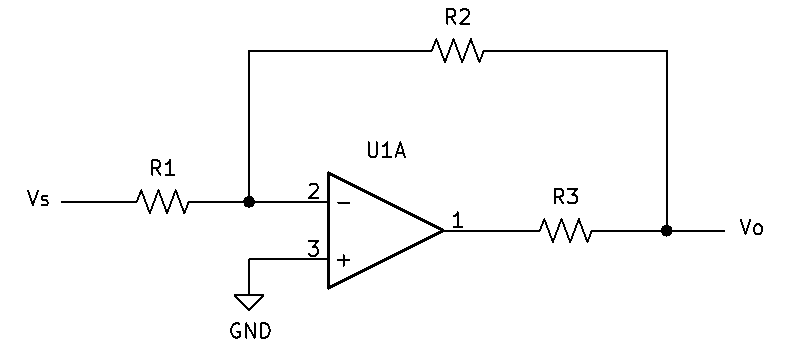
\includegraphics[scale=1]{figure1}
		\caption{Amplificador inversor con resistencia en la salida}
		\label{fig:pic1}
	\end{figure}
	
	Para analizar su ganancia de voltaje y corroborar si esta resistencia afecta o no, sustituimos el modelo ideal del amplificador operacional  por el circuito equivalente de un amplificador no ideal con el fin de poder emplear las leyes de Kirchhoff en el análisis del cicuito.
	En la figura \ref{fig:pic2} se muestra el circuito equivalente del amplificador inversor, debe tenerse en cuenta que en la resistencia $R_o$ se encuentra modelada la resistencia $R_3$ y la resistencia $R'_{o}$.
	
	Aplicando la LCK en el nodo $V_1$ obtenemos:
	\begin{equation}
		I_1 = I_2 + I_d
	\end{equation}

	Usando la ley de Ohm obtenemos
	\begin{align}
		\frac{ V_s - V_1 }{ R_1 } = \frac{ V_1 - V_o }{ R_2 } + \frac{ V_1 }{ R_d }\nonumber\\
		\frac{ V_s }{ R_1 } - \frac{ V_1 }{ R_1 } = \frac{ V_1 }{ R_d } + \frac{ V_1 }{ R_2 }\nonumber\\
		\left( \frac{1}{R_1}  + \frac{1}{R_2} + \frac{1}{R_d} \right)V_1 = \frac{V_s}{R_1} + \frac{V_o}{R_2}\nonumber\\
		\left( \frac{ R_2R_d + R_1R_d + R_1R_2 }{ R_1R_2R_d } \right)V_1 = \frac{V_s}{R_1} + \frac{V_o}{R_2}\nonumber
	\end{align}

	Por lo tanto
	\begin{align}
		\label{E:eq2}
		V_1 = \left( \frac{ R_1R_2R_d }{ R_2R_d + R_1R_d + R_1R_2 } \right)  \left( \frac{V_s}{R_1} + \frac{V_o}{R_2}\right)
	\end{align}

	\begin{figure}[H]
		\centering
		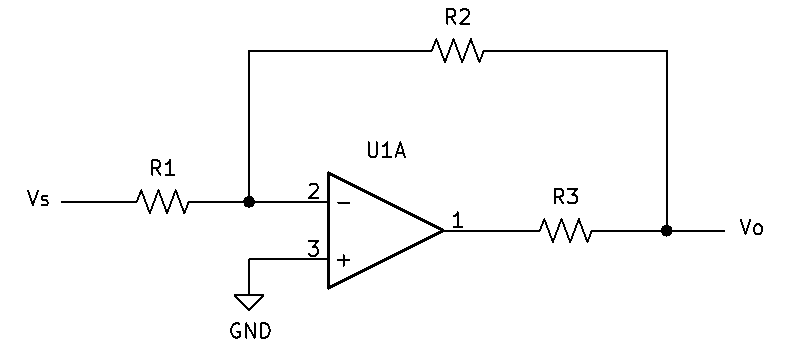
\includegraphics[scale=1]{figure1}
		\caption{Modelo equivalente para el amplificador inversor.}
		\label{fig:pic2}
	\end{figure}
	
	Aplicando ahora la LCK en el nodo $V_o$ del circuito de la figura \ref{fig:pic2} obtenemos:
	\begin{align}
		I_2 = I_o
	\end{align}

	O bien
	\begin{align}
		\label{E:eq4}
		\frac{V_1 - V_o}{R_2} = \frac{V_o - AV_d}{R_o}\nonumber\\
		\frac{V_1}{R_2} - \frac{V_o}{R_2} = \frac{V_o}{R_o} - \frac{AV_d}{R_o}  
	\end{align}

	No obstante, tenemos que
	\begin{align}
		\label{E:eq5}
		V_d = - V_1
	\end{align}

	La sustitución de la ecuación (\ref{E:eq5}) en la ecuación (\ref{E:eq4}) produce
	\begin{align}
		\frac{V_1}{R_2} - \frac{V_o}{R_2} = \frac{V_o}{R_o} + \frac{AV_1}{R_o}\nonumber\\
		\left( \frac{1}{R_o} + \frac{1}{R_2} \right)V_o = \left( \frac{1}{R_2} - \frac{A}{R_o} \right)V_1\nonumber\\
		\left( \frac{R_2 + R_o}{R_2R_o} \right)V_o = \left( \frac{R_o - AR_2}{R_2R_o} \right)V_1\nonumber\\
		V_o = \left( \frac{R_2R_o}{R_2 + R_o} \right) \left( \frac{R_o - AR_2}{R_2R_o} \right)V_1\nonumber
	\end{align}

	Por tanto
	\begin{align}
		\label{E:eq6}
		V_o = \left( \frac{R_o - AR_2}{R_2 + R_o} \right)V_1
	\end{align}

	Sustituimos la ecuación (\ref{E:eq2}) en la ecuación (\ref{E:eq6})
	\begin{align}
		\label{E:eq}
		V_o = \left( \frac{R_o - AR_2}{R_2 + R_o} \right)\left( \frac{ R_1R_2R_d }{ R_2R_d + R_1R_d + R_1R_2 } \right)  \left( \frac{V_s}{R_1} + \frac{V_o}{R_2}\right)\nonumber\\\nonumber\\
		V_o = \frac{Vs}{R_1}\left[\frac{R_1R_2R_d(R_o - AR_2)}{(R_2 + R_o)(R_2R_d + R_1R_d + R_1R_2)}\right] + \frac{V_o}{R_2}\left[\frac{R_1R_2R_d(R_o - AR_2)}{(R_2 + R_o)(R_2R_d + R_1R_d + R_1R_2)}\right]\nonumber\\\nonumber\\
		V_o = \frac{R_2R_d(R_o - AR_2)V_s}{(R_2 + R_o)(R_2R_d + R_1R_d + R_1R_2)} + \frac{R_1R_d(R_o - AR_2)V_o}{(R_2 + R_o)(R_2R_d + R_1R_d + R_1R_2)}\nonumber\\\nonumber\\
		\left[ 1 - \frac{R_1R_d(R_o - AR_2)V_s}{(R_2 + R_o)(R_2R_d + R_1R_d + R_1R_2)} \right]V_o = \frac{R_2R_d(R_o - AR_2)V_s}{(R_2 + R_o)(R_2R_d + R_1R_d + R_1R_2)}\nonumber\\\nonumber\\
		(R_2 + R_o)(R_2R_d + R_1R_d + R_1R_2) - (R_1R_d)(R_o - AR_2)V_o = R_2R_d(R_o - AR_2)V_s\nonumber
	\end{align}
	\begin{multline*}
		R_dR_2^{2} + R_1R_2R_d + R_1R_2^{2} + R_oR_2R_d + R_oR_1R_d + R_oR_1R_2\\ - R_oR_1R_d + AR_1R_2R_d)V_o = R_2R_d(R_o - AR_2)V_s
	\end{multline*}
	\begin{align}
		R_dR_2^{2} + R_1R_2R_d + R_1R_2^{2} + R_oR_2R_d + R_oR_1R_2 + AR_1R_2R_d)V_o = R_2R_d(R_o - AR_2)V_s\nonumber\\\nonumber\\
		R_2(R_2R_d + R_1R_d + R_1R_2 + R_oR_d + R_oR_1 + AR_1R_d)V_o = R_2R_d(R_o - AR_2)V_s\nonumber
	\end{align}
	\begin{align}
		\frac{V_o}{V_s} = \frac{R_d(R_o - AR_2)}{R_2R_d + R_1R_d + R_1R_2 + R_oR_d + R_oR_1 + AR_1R_d}
	\end{align}

	\vspace{0.5cm}
	
	Calculamos la ganancia de voltaje cuando $R_d \rightarrow \infty$
	\begin{align}
		\lim_{R_d \to \infty} \frac{V_o}{V_s} = \frac{R_o - AR_2}{\frac{R_1R_2 + R_oR_1}{R_d} + R_1 +R_2 + R_o + AR_1} = \frac{R_o - AR_2}{R_1 + R_2	+ R_o + AR_1}
	\end{align}
	 
	Ahora, si asumimos que la ganancia $A \rightarrow \infty$ la ganancia de voltaje se vuelve
	\begin{align}
		\lim_{A \to \infty} \frac{V_o}{V_s} = \frac{ \frac{R_o}{A} - R_2 }{ \frac{R1 + R_2 + R_o}{A} + R_1} = -\frac{R_2}{R_1}
	\end{align}

	De esta manera observamos que la resistencia $R_3$ entre la salida y el lazo de realimentación no afecta en lo absoluto la ganancia del voltaje del circuito.  Ahora, veremos como afecta la impedancia de salida, para esto nos remitimos al circuito de la figura 3 en donde la fuente de entrada se a cortocircuitado y se ha inyectado una fuente de corriente $I_X$.
	
	
	\begin{align}
		L = \frac{V_{OUT}}{f_s \times \Delta_{IL}} \left( 1 - \frac{V_{OUT}}{V_{IN}} \right) = \frac{\qty{5}{\volt}}{\qty{910}{\kilo \hertz} \times \qty{0.48}{\ampere}} \left( 1 - \frac{\qty{5}{\volt}}{\qty{24}{\volt}} \right) = \qty{9.062}{\micro \henry} \approx \qty{9.1}{\micro \henry}
	\end{align}
	
	
	\begin{align}
		f_s (kHz) = e^{\frac{ \ln \left( \frac{180000}{R_{freq}(k\Omega)} \right) }{1.1}}
	\end{align}
	
	\begin{align}
		f_s (kHz) = e^{\frac{ \ln \left( \frac{180000}{100} \right) }{1.1}} = \qty{910.62}{\kilo \hertz} \approx \qty{910}{\kilo \hertz}
	\end{align}
	
	\begin{align}
		\Delta I_L = \frac{V_{OUT}}{L \times f_{sw}} \left( 1 - \frac{V_{OUT}}{V_{IN}} \right) = \frac{\qty{5}{\volt}}{\qty{15}{\micro \henry} \times \qty{910}{\kilo \hertz}} \left( 1 - \frac{\qty{5}{\volt}}{\qty{24}{\volt} } \right) = \qty{0.28998779}{ \ampere}
	\end{align}
	
	\begin{align}
		R_{SENSE_{MAX}} < \frac{V_{SP} - V_{REF}}{I_{MAX} \times GAIN} \nonumber
	\end{align}
	
	\begin{align}
		R_{SENSE_{MIN}} > \frac{V_{SN} - V_{REF}}{I_{MIN} \times GAIN} \nonumber
	\end{align}
	
	
		\begin{align}
		\frac{V_{SN} - V_{REF}}{I_{MIN} \times GAIN} < R_{SENSE} < \frac{V_{SP} - V_{REF}}{I_{MAX} \times GAIN} \nonumber
	\end{align}
	
		\begin{align}
		V_{OUT} = I \times R_{SENSE} \times GAIN \nonumber
	\end{align}
	
			\begin{align}
		I = \frac{V_{OUT}}{R_{SENSE} \times GAIN}
	\end{align}
	
			\begin{align}
		\frac{V_{SN} - V_{REF}}{I_{MIN} \times GAIN} &< R_{SENSE} < \frac{V_{SP} - V_{REF}}{I_{MAX} \times GAIN} \nonumber \\
		\frac{\qty{0.05}{\milli \volt} - \qty{0}{\volt}}{\qty{1}{\micro \ampere} \times 25} &< R_{SENSE} < \frac{\qty{5}{\volt} - \qty{20}{\milli  \volt}}{\qty{100}{\micro \ampere} \times 25} \nonumber \\
		\qty{2}{\Omega} &< R_{SENSE} < \qty{1992}{\Omega}
	\end{align}
	
\end{document} 